\subsubsection{Correctitud}

Como mencionamos en la introducción, modelaremos el problema mediante grafos. Cada ciudad será representada con un grafo donde sus esquinas corresponden a los vértices y sus calles a las aristas respectivamente. \\
A lo largo de esta sección vamos a desarrollar un algorítmo que resuelva el problema. Para ello utilizaremos algunas propiedades que demostraremos a continuación, pero antes algunas definiciones que necesitaremos.

\begin{definition}
Sea $G=(V_g,X_g)$ un grafo, definimos como una \textbf{componente conexa} de $G$ al subgrafo conexo maximal de $G$
\end{definition}

\begin{definition}
Sea $G=(V_g,X_g)$ un grafo, y sea $e \in X_g$ una arista de $G$. Decimos que $e$ es un \textbf{puente} si y sólo al quitar dicha arista, la cantidad de componentes conexas de $G$ aumenta.
\end{definition}

Definido el concepto de puente de un grafo, enunciamos y demostramos el siguiente teorema que es la base de nuestro algoritmo.

\begin{lemma}
Sea $G=(V_g,X_g)$ un grafo conexo y sean v,w $\in$ $V_g$. $G$ no tiene puentes $\Rightarrow$ $\exists$ $C_1$, $C_2$ caminos de v a w tal que $C_1$ $\cap$ $C_2$ = $\emptyset$
\end{lemma}

\begin{proof}
Demostraremos el lema por contrarecíproco. Supongamos existen $k$ caminos distintos entre $v$ y $w$ tales que $\forall$ $C_i$ ($i \in \{1,\ldots,k\}$) , $\bigcap$ $C_i$ $\neq$ $\emptyset$. 
Entonces todos los caminos comparten al menos una arista. Sea $e \in X_g$ dicha arista, si la quitamos de $G$, no podremos alcanzar a $w$ desde $v$ (o viceversa) por ninguno de los caminos. 
Entonces $e$ es un puente, y por lo tanto $G$ tiene al menos un puente.  $\blacksquare$
\end{proof}

\begin{theorem}
Sea $G=(V_g,X_g)$ un grafo conexo. G no tiene puentes $\Longleftrightarrow$ Existe una forma de orientar a G tal que resulte fuertemente conexo.
\end{theorem}

\begin{proof}
Demostramos ambas implicaciones por separado. \\
$\Rightarrow$)
La siguiente demostración es constructiva. Veremos como ir asignando sentidos a las aristas de forma tal de finalizar con un grafo fuertemente conexo. \\
Sea $G$ un grafo conexo y sin puentes. Por el lema anterior sabemos que existen dos caminos disjuntos entre dos vértices inciales cualesquiera $v_0$ y $v_1$. 
Asignamos un sentido a uno de los caminos, y el inverso al otro, obteniendo un ciclo que puede o no incluir a mas vértices además de $v_0$ y $v_1$. \\
Luego aplicamos el siguiente proceso iterativamente:\\
\begin{itemize}
  \item Elegir un vértices $w$ que sea vecino de algún vértice $v$ que esté incluído en el ciclo orientado. Como el grafo $G$ no contiene puentes, no puede ocurrir que $d(w)=1$.
  \item Luego orientamos la arista que une a $v$ con $w$ con el sentido $v\rightarrow w$.
  \item Finalmente, orientamos alguna de las otras aristas incidentes a $w$, de forma tal de que el camino termine en algún vértice ya visitado por el ciclo orientado, o no. En el caso de que 
	no sea así, entonces vamos armando un camino orientado sin ciclos que parte de $w$ y eventualmente llegará a algún vértice que pertenece a un camino orientado.
\end{itemize}
El proceso termina pues la cantidad de vértices es finita, y al finalizar, tenemos orientadas casi todas las aristas de forma tal de poder ir de cualquier vértice a cualquier otro. Si quedan 
aristas sin orientar, se les da cualquier orientación y entonces tenemos a $G$ totalmente orientado, y resulta fuertemente conexo. \\ 

$\Leftarrow$)
Probamos el contrarecíproco.\\
Sea $G=(V_g, X_g)$ un grafo conexo con al menos un puente $e \in X_g$. Sean además $G_1, G_2$ las componentes conexas que quedan al quitar el puente $e$. Si tomamos dos nodos $v \in G_1$ y 
$w \in G_2$, la única forma de formar un camino de $v$ a $w$ es pasando por $e$, por lo que al orientar $e$ en algún sentido, ya no podrá ser posible encontrar un camino que nos lleve de $w$ a $v$. 
Entonces no es posible orientar a $G$ de forma tal que resulte fuertemente conexo. $\blacksquare$
\end{proof}

Utilizando el teorema vemos que el problema de decidir si existe una forma de orientar a $G$ es equivalente al problema de encontrar puentes, y es éste el problema que resuelve nuestro algoritmo. 
Una implementación inmediata sería: \\

\begin{verbatimtab}
Puentes = {};
Para toda arista e del grafo G
    Quitar e de G
    Si G no resulta conexo, agregar e al conjunto Puentes

devolver Puentes
\end{verbatimtab}

Si bien el algoritmo anterior resuelve el problema, puede mejorarse si caracterizamos los vértices que tienen un puente incidente a ellos, y de esa forma acotar la cantidad de aristas para probar 
si son puentes. Para realizar dicha caracterización, vamos a basarnos en un recorrido del grafo por niveles, al estilo \textit{BFS}.

\begin{definition}
Sea $G=(V_g, X_g)$ un grafo conexo, y sea $v_0 \in V_g$ un vértice cualquiera del grafo. Decimos que cualquier otro vértice tiene nivel $k$ respecto a $v_0$ si y sólo si $d(v_0, v)=k$. 
Además a las aristas incidentes a $v$ las notamos como aristas de nivel $k-1$, $k$ y $k+1$, donde la arista de nivel $i$ conecta a $v$ con otro vértice de nivel $i$.

\begin{center}
 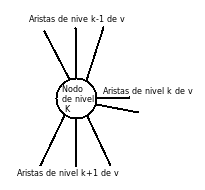
\includegraphics{img/ej2/nodo_nivel_k.png}
\end{center}
\end{definition}

Con un algoritmo BFS podemos empezar por cualquier vértice, y como es conexo, recorrer todos asignando el nivel respecto al vértice inicial. Nos interesa entonces poder decidir 
rápidamente si una arista es puente o no, sin tener que quitarla y verificar la conexidad del nuevo grafo sin ella. Para eso nos valdremos de la siguiente propiedad:

\begin{proposition}
Sea un grafo conexo $G=(V_g, X_g)$, tal que se asignan niveles a sus vértices respecto de algún $v_0$, y sea un vértice $v$ de nivel $k$ respecto a $v_0$. Las aristas de nivel $k$ de $v$ no son puentes. 
Además, si existen dos o más aristas de nivel $k-1$, entonces ninguna de ellas es puente. (Nota: las aristas de nivel $k+1$ para $v$ serán aristas de nivel $k$ para algún vértice de nivel $k+1$)
\end{proposition}

\begin{proof}
Sea $v$ un vértice de nivel $k$ respecto a $v_0$, y sea $e$ una arista de nivel $k$ para $v$, es decir, que une a $v$ con otro vértice del mismo nivel, llamémoslo $w$. Desde $v_0$ podemos ir a cualquier 
vértice del grafo por ser éste conexo. En particular podemos ir a $v$ y a $w$ por caminos que no usan la arista $e$, porque si hubiera que usarala, $w$ sería un nivel mayor. Entonces al quitar 
$e$ no aumenta la cantidad de componentes conexas de $G$, y por lo tanto $e$ no es un puente. \\
Ahora supongamos que $v$ tiene al menos dos aristas de nivel $k-1$. Sean $e_1$ y $e_2$ estas aristas, si quitamos $e_1$, desde $v$ todavía podemos ir al nivel $k-1$ usando $e_2$, y por 
lo tanto, llegar hasta $v_0$ y desde ahí alcanzar el nodo que era vecino de $v$ mediante $e_1$. El caso es análogo si quitamos $e_2$. Nuevamente quitar una de estas aristas no hace que aumente 
la cantidad de componentes conexas de $G$, por lo tanto ninguna es puente. $blacksquare$ 
\end{proof}

Con esta propiedad entonces podemos evitar tener que probar con todas las aristas. Sólo basta revisar aquellas aristas que, eligiendo un $v_0$, son de nivel $k-1$ para algún vértice $v$ de nivel 
$k$ respecto a $v_0$ y $v$ no tiene más aristas de nivel $k-1$. Entonces nuestro algoritmo queda expresado de la siguiente forma:

\begin{verbatimtab}
Puentes 	= {}
PosiblesPuentes = {}

Elegir un v_0 de G

Para todo v en G
    Si v es de nivel k y tiene una sola arista e de nivel k-1, agregar e a PosiblesPuentes

Para toda arista e en PosiblesPuentes
    Quitar e de G
    Si G es no conexo, agregar e a Puentes

devolver Puentes
\end{verbatimtab}

Si el algoritmo encuentra al menos un puente, entonces no es posible orientar al grafo para que resulte fuertemente conexo. Si el conjunto devuelto es vacío, entonces si es posible. Hemos demostrado 
la correctitud de nuestro algoritmo. \\

\subsubsection{Complejidad}
Analizaremos ahora la complejidad computacional de nuestro algoritmo.\\

Elegir un nodo para comenzar a asignar niveles se realiza en $O(1)$. \\
El recorrido por niveles de los nodos lo realizamos con un algoritmo BFS

\begin{verbatimtab}
Cola 	= {}

Asignar nivel 0 a v_0
Encolar v_0 en Cola

Mientras haya vertices en Cola
{
    Poner en v el primero de Cola
    Para todo vecino w de v
    {
	Si w no tiene nivel asignado
	{
	    Asignar a w el nivel de v + 1
	    Encolar w en Cola
	}
    }
}
\end{verbatimtab}

Por cada vértice, si no fue visitado antes (es decir, no tiene nivel asignado), encolamos en $O(1)$ a cada uno de sus vecinos. Cada vértice $v$ tiene $d(v)$ vecinos, por lo que el costo 
total de revisar a todos los nodos es 
\begin{center}
 $\sum_{i=1}^{n} d(v_i) = 2m = O(m)$
\end{center}
Encolar una arista si el vértice sólo tiene un vecino de un nivel menor se hace en $O(1)$, por lo que la complejidad de la primera parte de nuestro algoritmo es $O(m)$.\\

Ahora resta recorrer el conjunto de posibles aristas puente y probar una por una si la cantidad de componentes conexas aumenta al quitarla. \textbf{En el peor caso}, la cantidad de aristas en el 
conjunto es n-1, ya que el primer nodo $v_0$ nunca tiene aristas de nivel inferior a su propio nivel. Notemos que no puede haber más de n-1 porque en ese caso habría un vértice que tendría 
por lo menos 2 o más aristas de nivel menor y entonces no serían puentes ninguna de ellas. Para probar la conexidad de un grafo utilizamos el mismo algoritmo BFS anterior, aunque 
sólo nos importa que la cantidad de vértices marcados como visitados sea $n$ al final del proceso, por lo que comprobar si $G$ es conexo es $O(m)$. Luego la complejidad total de verificar 
cada arista es $O(nm)$. \\
Antes de concluir, hacemos notar un detalle. El proceso de quitar una arista del grafo $G$ no es $O(1)$, sino que es $O(2 log (n-1))$ ya que en nuestra implementación, cada nodo guarda a 
sus vecinos en una estructura de datos \footnote{Utilizamos el contenedor \textit{set} de la STL de C++} que permite agregar o quitar elementos en tiempo proporcional al logaritmo de la 
cantidad de elementos. Como cada vértice tiene a lo sumo $n-1$ vecinos, y como cada arista une dos vértices, quitar un vecino por cada uno de los dos vértices se realiza en $O(2 log(n-1))$. 
Sin embargo, en términos de complejidad, vemos que no nos afecta ya que $m=O(n^2)$

\begin{center}
 $O(n(2log(n-1) + m)) = O(2nlog(n-1) + nm) = O(nm)$
\end{center}

Finalmente la complejidad de nuestro algoritmo es $O(nm)$, que es estrictamente menor que la primera aproximacion que habíamos propuesto en $O(m^2) = O(n^4)$.